\begin{figure}
  \centering
  \captionsetup{justification=centering}
  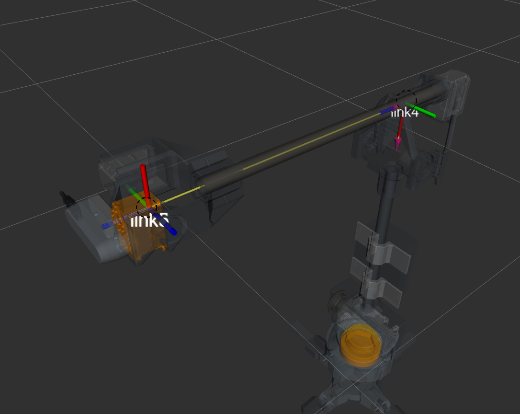
\includegraphics[width=\linewidth]{\thesisDir/chapter3/figures/r_mini_pieper.png}
  \caption{Rimini wrist conforms to Pieper condition where axis of rotation 
  for joint4, joint5, and joint6 share points of intercept. The dash circle in the 
  diagram a possible point of intercepts. Both point are valid for a Pieper condition}
  \label{fig:r_mini_pieper}
\end{figure}

